\subsection{Stochastic Volatility}\label{ssec:stochastic_volatility}

\begin{figure*}[t]
    \centering
    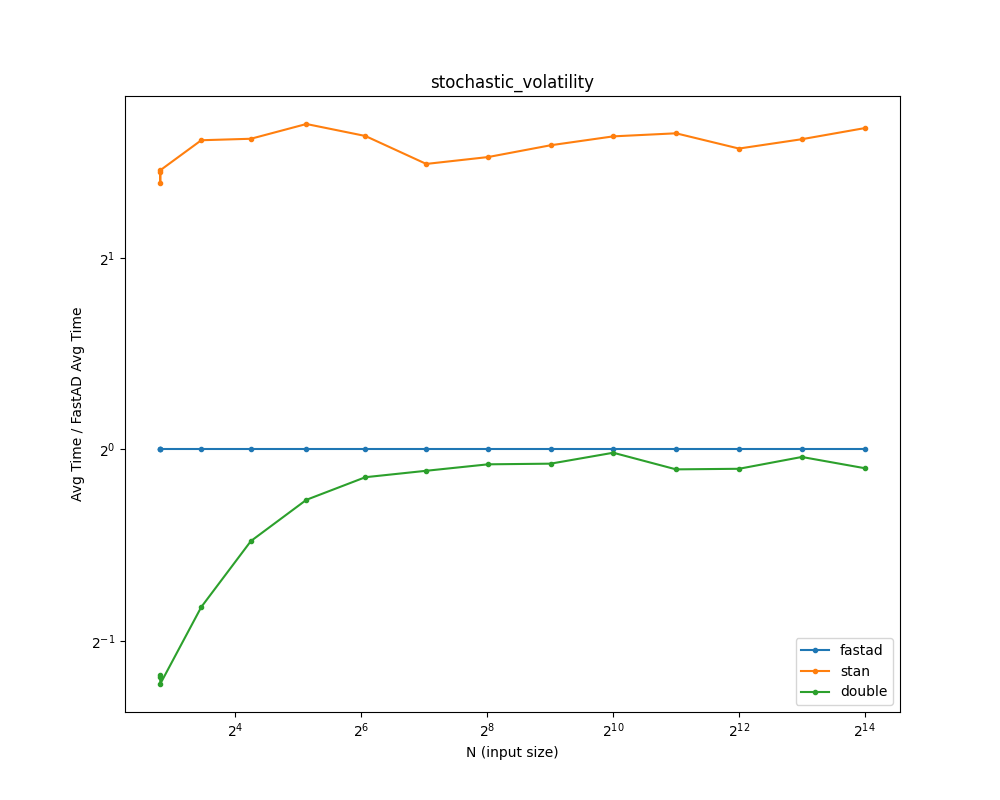
\includegraphics[width=\textwidth]{figs/stochastic_volatility_fig.png}
    \caption{%
        Stochastic volatility benchmark of Stan against FastAD 
        plotted relative to FastAD average time.
    }\label{fig:stochastic_volatility}
\end{figure*}

This section marks the second and last macro-benchmark example.
We consider the following stochastic volatility model 
taken from \todo{how to cite Stan documentation?}:
\begin{align*}
    y &\sim N(0, e^{h}) \\
    h_{std} &\sim N(0, 1) \\
    \sigma &\sim Cauchy(0,5) \\
    \mu &\sim Cauchy(0,10) \\
    \phi &\sim Unif(-1, 1) \\
    h &= h_{std} \cdot \sigma \\
    h[0] &= \frac{h[0]}{\sqrt{1 - \phi^2}} \\
    h &= h + \mu \\
    h[i] &= \phi \cdot (h[i-1] - \mu),\, i > 0
\end{align*}
The target function is the log of the joint probability density function (up to a constant)
and we wish to differentiate it with respect to $h_{std}, h, \phi, \sigma, \mu$.
For this benchmark, we only consider Stan for the same reasons described in Section~\ref{ssec:regression}.
The fill function for this functor will resize a vector of size $N$ as $\tilde{N} = N + 3$,
where the first $N/2$ values refer to $h_{std}$,
the next $N/2$ values refer to $h$,
and the next three refer to $\phi, \sigma, \mu$, respectively.
We take care of the edge case where $N < 2$ to let $N = 2$ and then carry out the steps above.
Here, $y$ is a constant.
All quantities are random generated uniformly in $(-1,1)$ range,
but $\sigma$ is replaced with its absolute value plus $0.1$ to make it strictly positive.

The following is the Stan functor overload:
\begin{lstlisting}[style=customcpp]
    using namespace stan::math;
    using vec_t = Eigen::Matrix<var, Eigen::Dynamic, 1>;
    size_t N = (x.size() - 3) / 2;
    Eigen::Map<vec_t> h_std(x.data(), N);
    Eigen::Map<vec_t> h(x.data() + N, N);
    auto& phi = x(2*N);
    auto& sigma = x(2*N + 1);
    auto& mu = x(2*N + 2);
    h = h_std * sigma;
    h[0] /= sqrt(1. - phi * phi);
    h += mu * Eigen::VectorXd::Ones(N);
    for (size_t i = 1; i < N; ++i) {
        h[i] += phi * (h[i-1] - mu);
    }
    auto lp = normal_lpdf(y, 0., exp(h / 2.)) +
            normal_lpdf(h_std, 0., 1.) +
            cauchy_lpdf(sigma, 0., 5.) +
            cauchy_lpdf(mu, 0., 10.) +
            uniform_lpdf(phi, -1., 1.);
\end{lstlisting}
The following is the FastAD functor overload:
\begin{lstlisting}[style=customcpp]
    size_t N = (x.size() - 3) / 2;
    ad::VarView<T, ad::vec> h_std(x.data(), x.data_adj(), N);
    ad::VarView<T, ad::vec> h(x.data() + N, x.data_adj() + N, N);
    ad::VarView<T> phi(x.data() + 2*N, x.data_adj() + 2*N);
    ad::VarView<T> sigma(x.data() + 2*N + 1, x.data_adj() + 2*N + 1);
    ad::VarView<T> mu(x.data() + 2*N + 2, x.data_adj() + 2*N + 2);
    auto tp = (
        h = h_std * sigma,
        h[0] /= ad::sqrt(1. - phi * phi),
        h += mu,
        ad::for_each(counting_iterator<>(1),
                     counting_iterator<>(N),
                     [&](size_t i) { return h[i] += phi * (h[i-1] - mu); })
    );
    auto lp = ad::normal_adj_log_pdf(y, 0., ad::exp(h / 2.)) 
            + ad::normal_adj_log_pdf(h_std, 0., 1.)
            + ad::cauchy_adj_log_pdf(sigma, 0., 5.)
            + ad::cauchy_adj_log_pdf(mu, 0., 10.) 
            + ad::uniform_adj_log_pdf(phi, -1., 1.);
    return (tp, lp);
\end{lstlisting}
Fig.\ref{fig:stochastic_volatility} shows the benchmark results.

FastAD outperforms Stan by 3 times for the largest $N$.
The trend seems quite stabilized from the start.
It is interesting to see that FastAD is only marginally slower than the \verb|double| baseline
for moderate to large $N$ values.
The ratio between FastAD time to baseline time is $ 1.07$, which means there is about a $7\%$ overhead only
from just one forward-evaluation to also compute the gradient.
Hence, gradient computation is almost free from just computing the log-pdf,
which puts FastAD at near-optimal performance.
